%----------------------------------------------------------------------------------------
%	SECTION 1.3
%----------------------------------------------------------------------------------------

\section{The Order Topology.}

\begin{definition}
    Let $X$ be a set with a simple order relation, and suppose that  $|X|>1$. Let $\Bc$ 
    be the collection of sets of the following forms:
        \begin{enumerate}[label=(\arabic*)]
            \item All open intervalcs $(a,b) \in X$.
                
            \item All half open intervals $[a_0,b)$ where $a_0$ is the least element 
                (if any) of $X$.

            \item All half open intervals of the form  $(a,b_0]$ where $b_0$ is the greatest 
                element (if any) of $X$.
        \end{enumerate}
    Then $\Bc$ forms the basis for a topology on  $X$ called the \textbf{order topology}
\end{definition}

\begin{theorem}\label{1.3.1}
    The collection $\Bc$ forms a basis.
\end{theorem}
\begin{proof}
    Consider $x \in X$, if  $x$ is the least element of  $X$, then it liess in all 
    intervals of type $(2)$, if it is the largest, then it lies in all intervals of type 
    $(3)$. If $x$ is neither the least nor largest element, then $x \in (a_0,b_0)$ with 
    $a_0$ and $b_0$ the least and largest elements (if any) of $X$. If no such elements 
    exist, then $x \in (a,b)$, for some lowerbound $a$ and upperbound $b$. Thus, in all three 
    cases, there is a basis element containing  $x$. 

    Now suppose $B_1,B_2 \in \Bc$ such that $x \in B_1 \cap B_2$. If $B_1$ and $B_2$ are 
    both of type $(1)$, then let  $B_1=(a,b)$, $B_2=(c,d)$, then $B_1 \cap B_2$ is an 
    open interval of type $(1)$, now fix  $B_1$ to be of type one. If $B_2$ is of type $(2)$, then 
    letting  $B_2=[a_0,c)$, then $x \in [a_0,d)$ for some $d \in X$. Likewise, if  $B_2=(c,b_0]$, 
    is of type $(3)$, we get a similar result. Moreover, the results are analogous if we 
    fix  $B_2$ and let $B_1$ range between intervals of the three types. Thusm in all cases, there 
    is a $B_3 \in \Bc$ such that $x \in B_3 \subseteq B_1 \cap B_2$.
\end{proof}

\begin{example}
    \begin{enumerate}[label=(\arabic*)]
        \item The standard topology on $\R$ is the order topology on $\R$ induced by the 
            usual order relation. We have that $\R$ under this topology has no intervals of 
            type  $(2)$, nor  $(3)$, so all bases elements in the standard topology are 
            open intervals in $\R$.

        \item Consider the dictionary order on  $\R \times \R$. Since  $\R \times \R$ has 
            no intervals of type $(2)$, nor $(3)$, the bases of  $\R \times \R$ under the 
            dictionary order are the open intervals of the form  $(a \times b, c \times d)$ Where 
             $a \leq c$, and  $b<d$.

             \begin{figure}
                 \centering
                 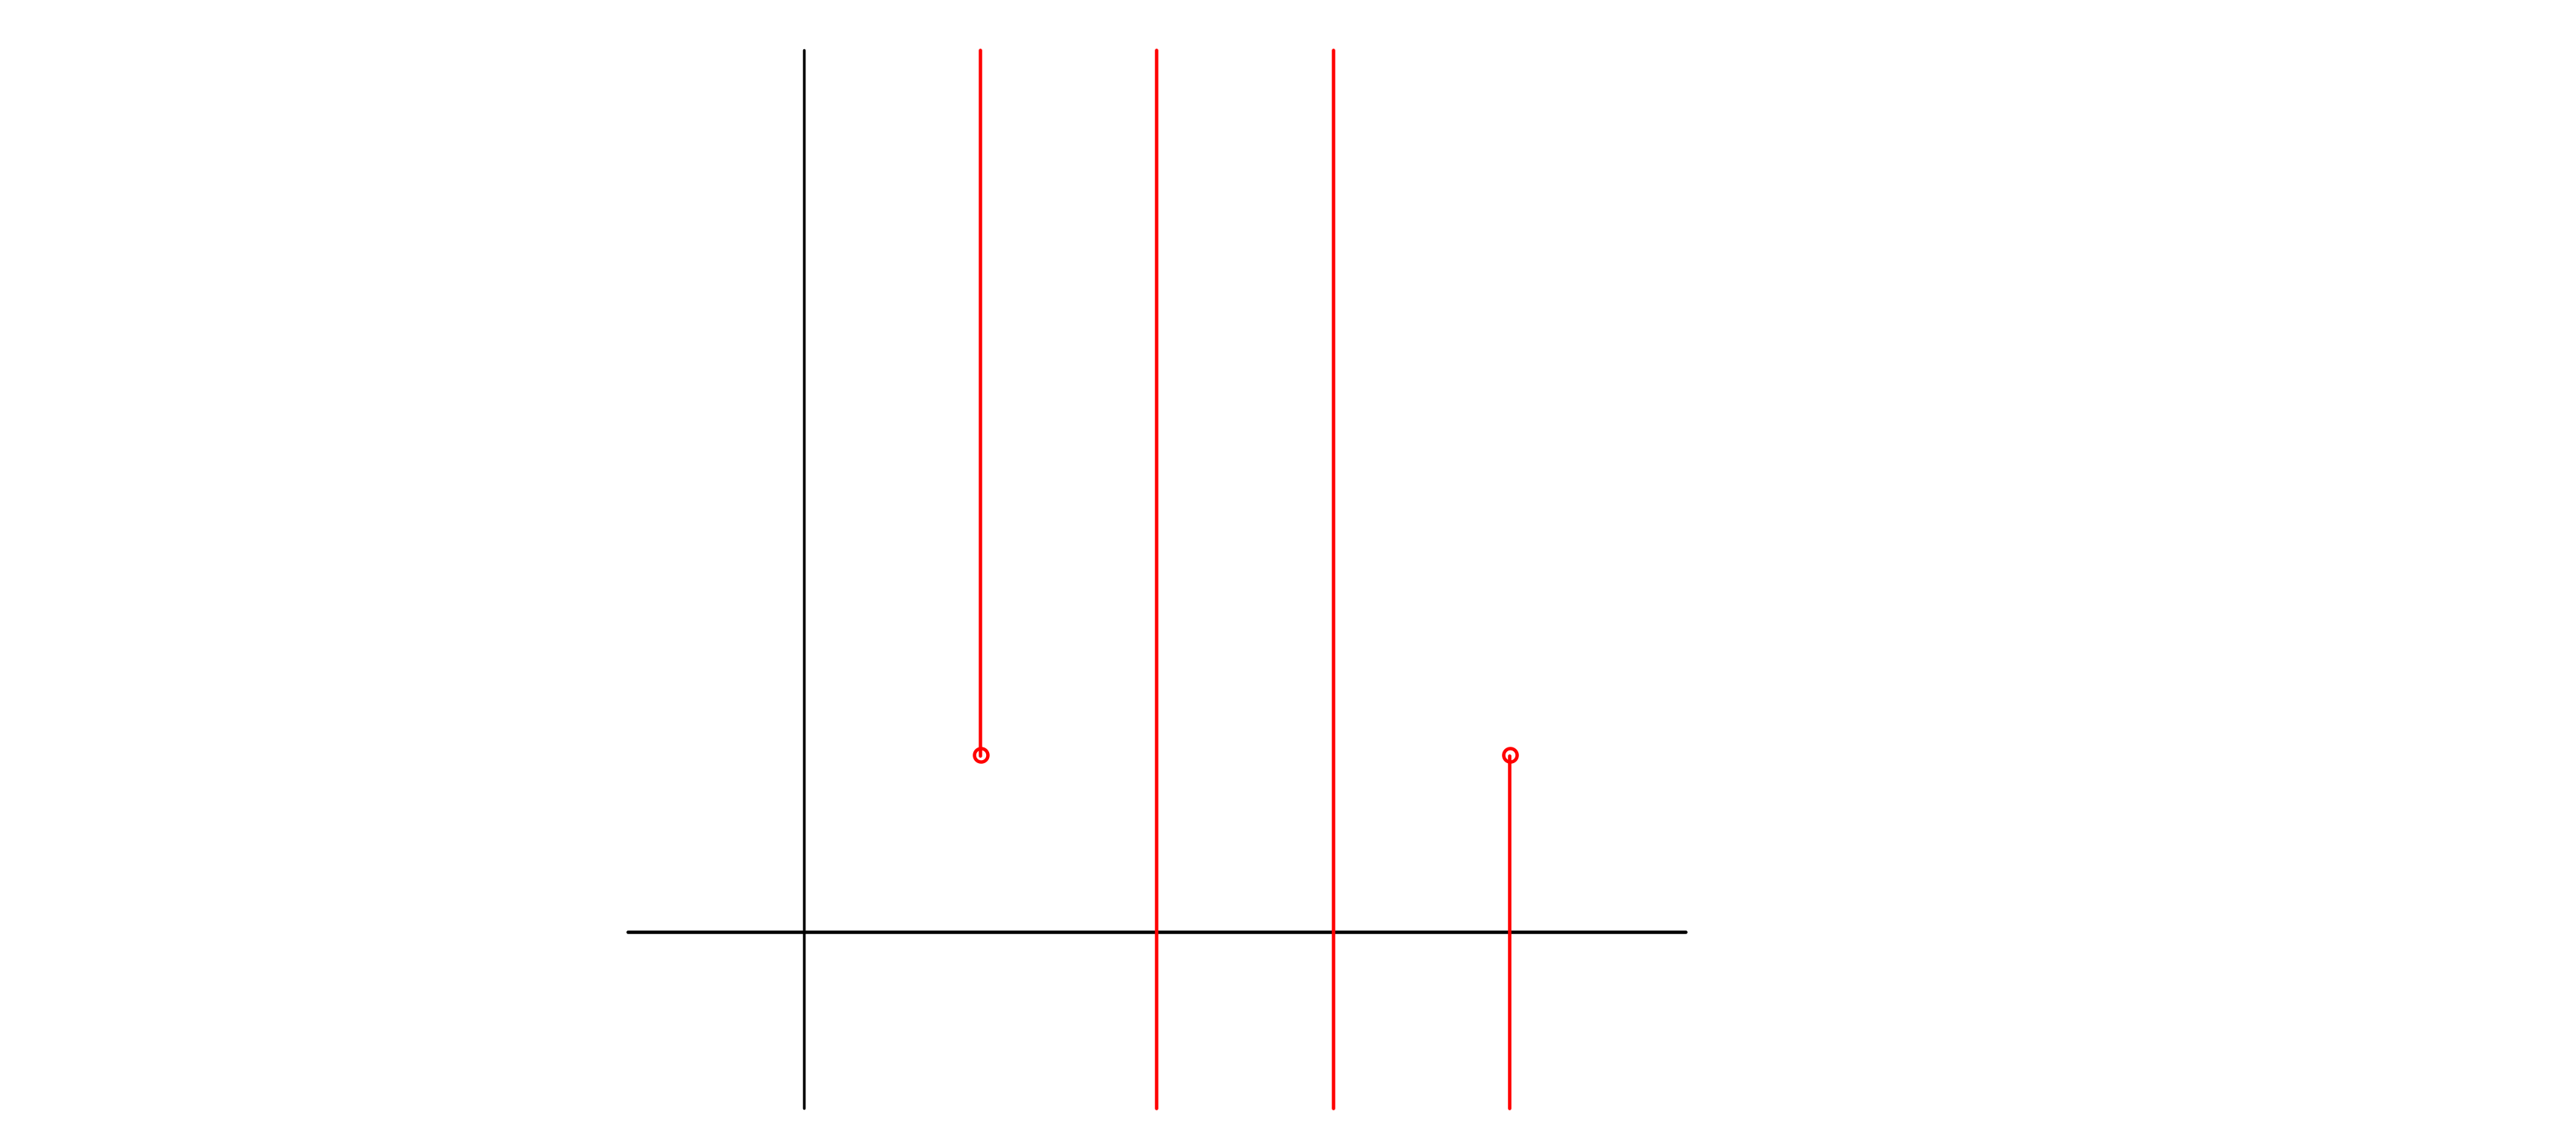
\includegraphics[scale = 0.3]{Figures/Chapter1/orderTopologyOnRxR.png}
                 \caption{The order topology on $\R \times \R$.}
                 \label{fig1.3}
             \end{figure}

         \item The positive integers  $\Z^+$ with the least element  $1$ form an ordered set 
             under the usual order. Taking  $n>1$, we see the bases of  $\Z^+$ under the order 
             topology are of the form  $(n-1,n+1)=\{n\}$ and $[1,n)=\{1, \dots ,n-1\}$. Thus 
             the order topology on  $\Z^+$ is the discrete topology.


         \item The set  $X=\{1,2\} \times \Z^+$ over the dictionary order is also an ordered set, 
             with the least elelment  $1 \times 1$. Denote  $1 \times n$ as  $a_n$ and  $2 \times n$ as 
              $b_n$. Then  $X$ consist of the elements  $a_1,a_2, \dots,b_1,b_2,\dots$.

              Now take $\{b_1\}$, then any open set containing $b_1$ must have a basis 
              about $b_1$, and also contains points $a_i$ with  $i \in \Z^+$; thus the 
              order topology on  $X$ is not the discrete topology.
    \end{enumerate}		
\end{example} 

\begin{definition}
    Let $X$ be an ordered set, and let  $a \in X$. There are two subsets in  $X$, 
    $(a,\infty)=\{x \in X: x>a\}$ and $(-\infty,a)=\{x \in X: x<a\}$ called \textbf{open rays} of $X$. 
    There are also two sets $[a,\infty)=\{x \in X: x \geq a\}$ and $(-\infty,a]=\{x \in X: x \leq a\}$ 
    called \textbf{closed rays} of $X$.
\end{definition}

\begin{theorem}\label{1.3.2}
    Let $X$ be an ordered set. Then the collection of all open rays in  $X$ form a subbasis 
    for the order topology on  $X$. 
\end{theorem}
\begin{proof}
    Let $\Sc$ be the collection of all open rays of  $X$, let  $(a,\infty)$ and  $(-\infty,b) \in \Sc$, 
    then  $(a,b)=(a,\infty) \cap (-\infty,b)$. Now take:
        \begin{equation*}
            S=\bigcup_{a,b \in X}{(a,b)}
        \end{equation*} 
    then $S \subseteq X$, likewise, since  $S$ runs through all intersections of open rays 
    of $X$, it contains all open intervals in  $X$, hence  $X \subseteq S$, and so  $X=S$ 
    as required.
\end{proof}
